\section{Design} \label{Design}

The PCAL geometry~\cite{2015002} is shown schematically in Fig.~\ref{fig:S3_1}. The
active area of PCAL is an isosceles triangle with a base length of $394$~cm and a base angle $\alpha=62.9^\circ$.
The apex of the triangle is nearest the beamline, while a line from the target point to the front face of each
module subtends an angle of $25^\circ$ with respect to the beamline. Each PCAL module is composed of 15
layers of 1~cm thick scintillator sandwiched with 14 layers of 0.22~cm thick lead, similar to the inner calorimeter of the CLAS EC~\cite{clas6nim}. Light generated in the scintillator strips by ionizing radiation is downconverted is using wavelength-shifting (WLS) fibers inserted inside holes running the length of the strips (see Fig.~\ref{fig:S3_4}). The fibers also transport the light to PMT housing adapters located along the base and U readout side of the triangle.  Each scintillator and lead layer is separated by a $50~\mu$m Teflon sheet and the entire
scintillator/lead volume is confined within a triangular shaped box. Note the EC uses a projective geometry
where each scintillator layer subtends the same solid angle as seen from the target, whereas the PCAL does
not. The PCAL active area is slightly larger than the acceptance of the EC, as indicated in Fig.~\ref{fig:S3_1} by projecting the EC towards the target through the location of the last layer of the PCAL. 

\begin{figure}[h]
\centering
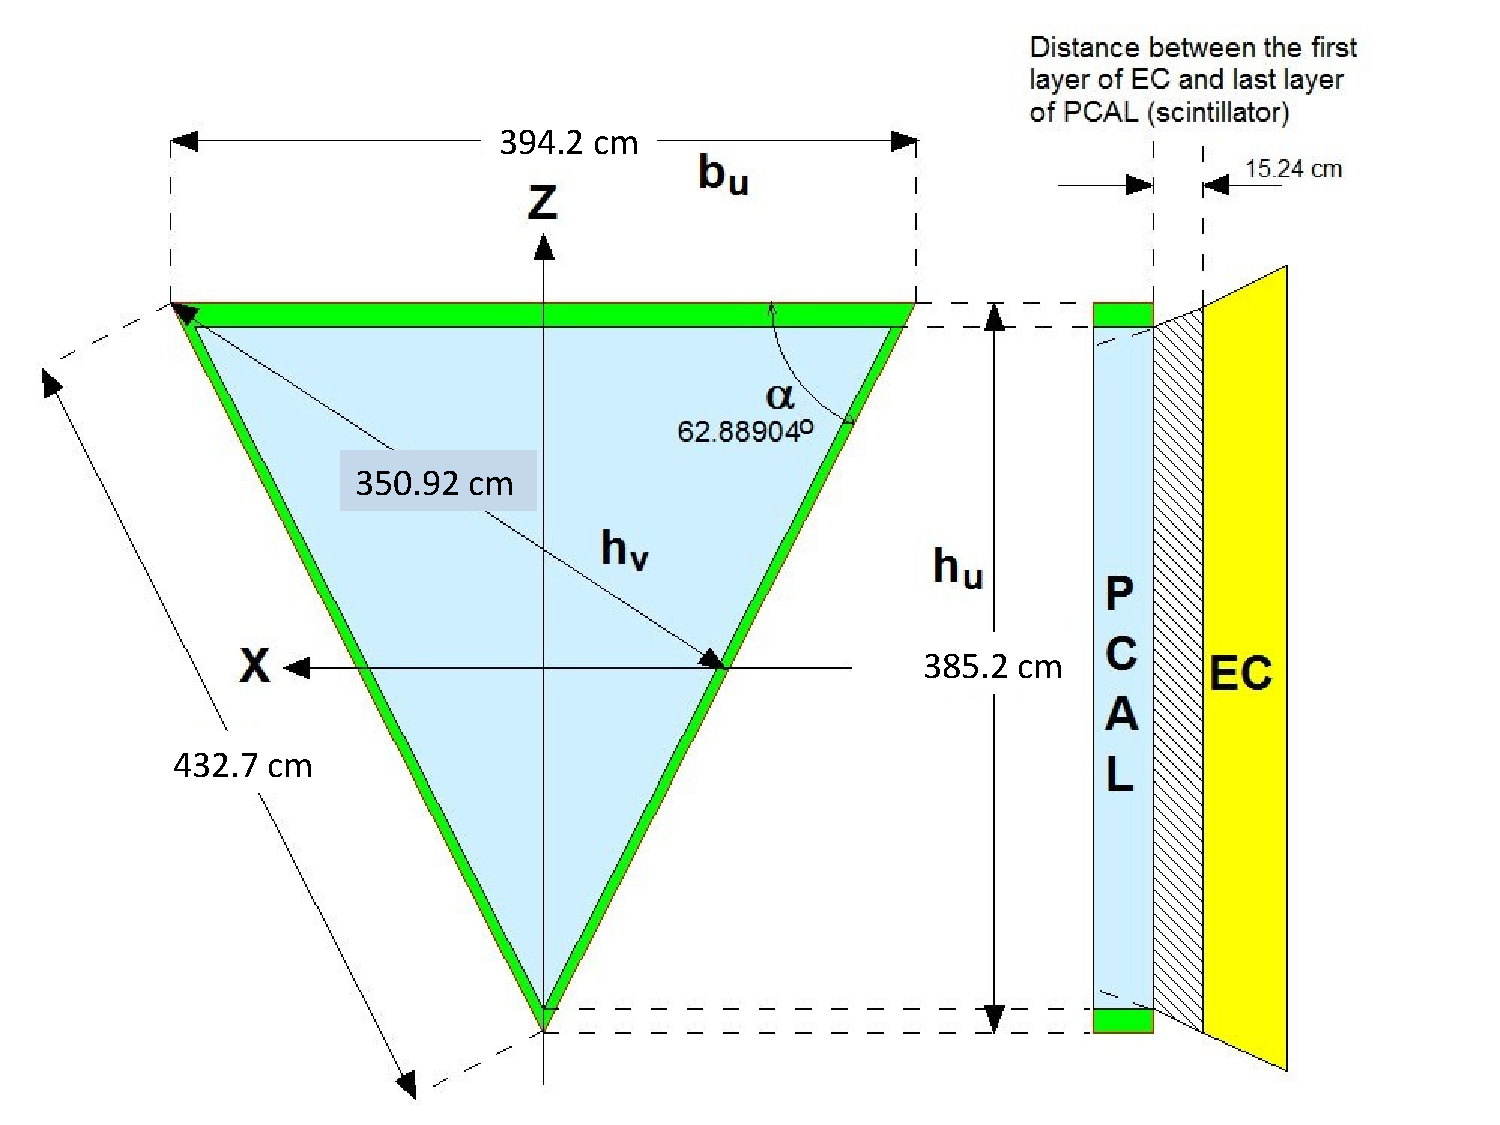
\includegraphics[width=1.0\columnwidth,keepaspectratio]{img/S3_1.pdf}
\caption[Schematic plot of PCAL]{A schematic view showing the dimensions of a PCAL module. The length
of the longest U scintillator strip at the base of the triangle is 394.2~cm and 432.7~cm for the V
and W strips along the sides of the triangle. }
\label{fig:S3_1}
\end{figure}


\begin{figure}[hbt]
\centering
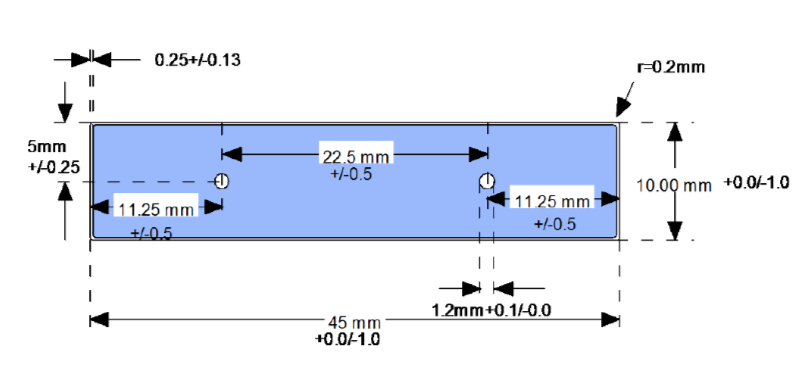
\includegraphics[width=1.05\columnwidth,keepaspectratio]{img/S3_4a.png}
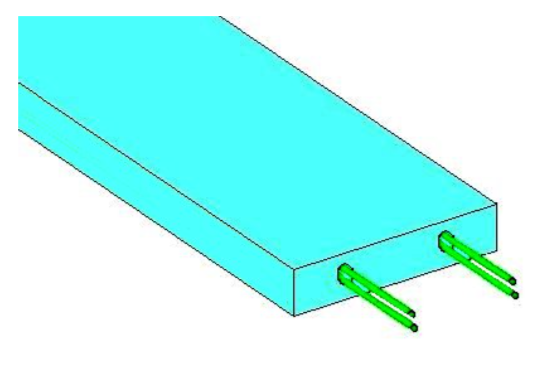
\includegraphics[width=0.75\columnwidth,keepaspectratio]{img/S3_4b.png}
\caption[PCAL UVW Layers]{Top: Design dimensions of the scintillator cross section. Bottom: Rendering of the
  strip with two fibers in each hole.}
\label{fig:S3_4}
\end{figure}

There are $84$ strips in each U-view layer, and $77$ strips in each of the V and W layers, for a total of 1190 scintillator strips installed in each of the six PCAL modules. Each scintillator has four WLS fibers for a total of 4760 installed and routed fibers per module. In order to optimize the number of
readout channels, each pair of strips at large scattering angles are combined into a single readout channel (fibers
from two adjacent strips are routed to a single PMT). For the first 52 shortest strips in U and for the last 46
longest strips in the V and W stereo readout planes the 4.5~cm (single strip) segmentation is used. For the
remaining strips, 9.0~cm wide (double strip) segmentation is used. Thus there are a total of 68 PMT readout
channels for U, and 62 for V and W.
